\section{Robustness, falsification and interpretation}
\begin{table}[htbp]\centering\small
\caption{Selected fifty-year hybrid robustness experiments}
\begin{tabular}{lllll}
\toprule
Experiment & MVI/GDP & Wealth Gini & Tax/GDP & Peak inflation \\
\midrule
baseline & 10.2\% & 0.584 & 27.1\% & 2.1\% \\
low relative floor & 0.0\% & 0.604 & 16.7\% & 2.1\% \\
high relative floor & 30.6\% & 0.549 & 48.0\% & 2.1\% \\
fixed real floor & 0.0\% & 0.605 & 16.7\% & 2.1\% \\
historical 33pct levy & 9.1\% & 0.589 & 23.4\% & 34.4\% \\
supply shock & 10.2\% & 0.584 & 27.1\% & 27.7\% \\
fiscal capacity limit & 10.0\% & 0.585 & 26.5\% & 9.5\% \\
low coverage & 19.1\% & 0.605 & 36.2\% & 2.1\% \\
score attack & 12.3\% & 0.624 & 29.3\% & 2.1\% \\
consumption scores & 14.3\% & 0.660 & 31.3\% & 2.1\% \\
equal grants comparator & 5.4\% & 0.560 & 22.3\% & 2.1\% \\
liquidation no vesting & 18.2\% & 0.753 & 35.2\% & 2.1\% \\
liquidation with vesting & 14.3\% & 0.663 & 31.3\% & 2.1\% \\
\bottomrule
\end{tabular}

\end{table}

An unanticipated 20\% supply disruption produces peak inflation around 27.66\% despite the adaptive rule. A 40\% liquidity-preference shock produces about 25.69\%. Optimistic output forecasting, a restrictive fiscal-capacity ceiling and the 33\% levy also break the narrow central price pattern. A feedback architecture must therefore be evaluated with forecast error and bounded instruments; deterministic target tracking is not robustness.

In the 128 paired parameter designs, B6 lowers the wealth Gini relative to B2 in all configurations. The median reduction is about 0.169 Gini units in this particular synthetic design. MVI/GDP is lower in 106 configurations and conventional tax/GDP in 124. Output is lower in 61, with the remaining cases generally limited by a common resource ceiling. Only six hybrid configurations meet the final-five-year MVI-below-1\% criterion, compared with four under B5 and none under B2. All 128 adaptive hybrid configurations remain within the defined 5\% annual price band, but the parameter box does not include the discrete supply and money-demand shocks that generate large inflation in the separate stress tests. These frequencies are not estimated probabilities of policy success.

\begin{figure}[htbp]\centering
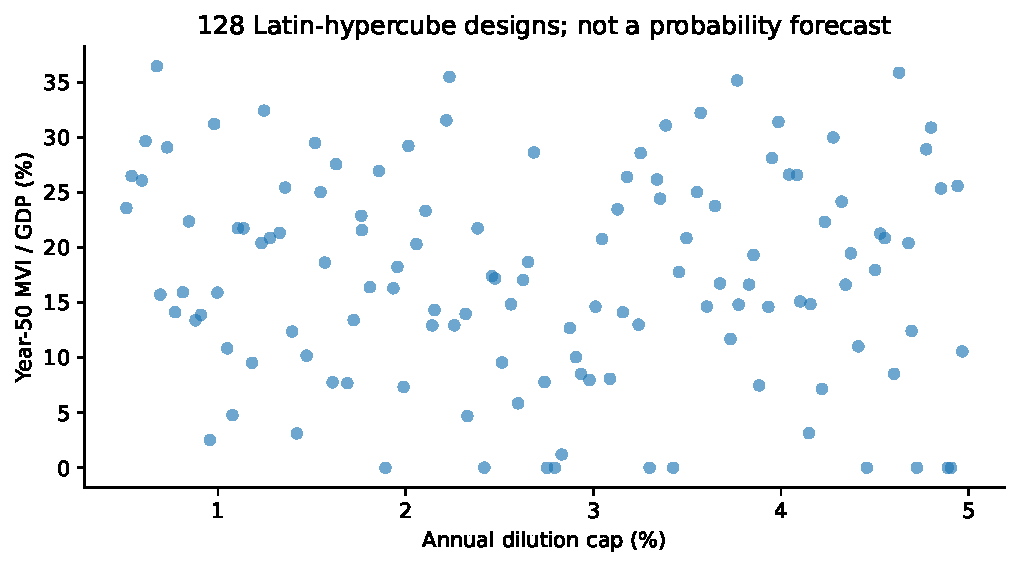
\includegraphics[width=.92\linewidth]{figures/sensitivity_scatter.pdf}
\caption{The transfer outcome depends on more than the dilution cap. The plotted Latin-hypercube box is exploratory, not a distribution of forecast uncertainty.}
\end{figure}

The results support a narrower set of hypotheses than the motivating proposal. Firm-specific equity can improve dispersion under the assumed grant rules, and enough broadly received capital income can replace a specified income top-up. The tests reject a universal claim that demurrage stabilises prices, an unconditional sunset, and the adequacy of aggregate ownership statistics as evidence of lower-tail coverage. They do not establish that a seigniorage-led bridge dominates a conventional tax-financed transition. In the successful monetary cases, flexible fiscal support is doing substantial stabilising work.

This separation also prevents a circular interpretation of the policy rule. If the government changes taxes until a desired money path is attained, low inflation is partly a consequence of the combined fiscal--monetary design. It cannot be cited as evidence that taxes were unnecessary. The relevant research question becomes how much of the transitional fiscal need can be safely allocated to monetary financing, given independent estimates of money demand and available fiscal capacity.

